%% Source: https://github.com/tias/constraint-solving-course
%% Licensed under CC BY-NC-SA 4.0: https://creativecommons.org/licenses/by-nc-sa/4.0/
%% You may share and adapt this for non-commercial use,
%% with attribution and under the same license.

\documentclass{cons-beamer}
\usepackage{cancel}
\usetikzlibrary{overlay-beamer-styles}

\begin{document}

\titleFrame{
	L06: Solving technologies and encodings, part 1
}{
	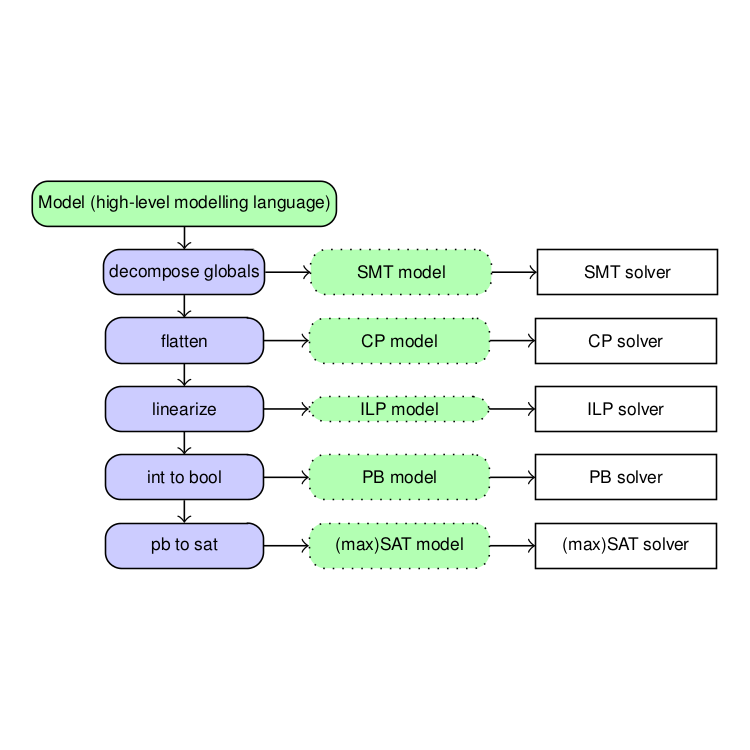
\includegraphics[height=42mm, trim=0 50pt 0 50pt, clip]{images/ch6-logo.png}
}{
	Partly based on slides from Pierre Flener and H\'{e}l\`{e}ne Verhaeghe.
}


\begin{frame}{Recap: search, inference and primitive constraints}
	From Lecture 1:\\
	Solving combinatorial problems \textbf{intelligently}:
	\begin{itemize}
		\item \search{Search}: Explore the space of possible assignments.
		\item \inference{Inference}: Reduce the space to feasible (partial) assignments.
	\end{itemize}
	\vfill

	From Lecture 3:\\
	\begin{definition}
		\textit{Primitive constraint}: a constraint that the solver can do  \inference{inference} with.
	\end{definition}
	
	For CP, PB and SAT \inference{inference=propagation}.
	
	\begin{definition}
		\textit{Propagation}: using the properties of a primitive constraint to \inference{reduce the domains} of participating decision variables by removing unsupported values.
	\end{definition}
	Example: $x + 2 \cdot y \geq 3, \quad D(x) = \{0,1,2\}, D(y) = \{0,1,2\}$ \\
	$\qquad \qquad \qquad \implies D(y) = \{\cancel{\red{0}},1,2\}$
\end{frame}

\begin{frame}{Recap: solvers and primitive constraints}
	Different solver paradigms have different \defined{primitive} constraints:
	\vfill
	
	\begin{itemize}\setlength\itemsep{1em}
		\item \textbf{Boolean SATisfiability solvers}: Clause: $b_1 \vee b_2 \vee ... \vee b_n$
		\item \textbf{Pseudo-Boolean solvers}: $\sum w \cdot b \;\lessgtr\; c$ \\
		\quad(with $w,c$ constant, $\;\lessgtr\; \in \{=,<,\leq,>,\geq\}$)
		\item \textbf{Integer Linear solvers}: $\sum w \cdot v \;\lessgtr\; c$ and $v \;\lessgtr\; c$ \\
		\quad(with $w,c$ constant, $\;\lessgtr\; \in \{=,\leq,\geq\}$)
	\end{itemize}
	\vfill
	
	\textbf{CP solvers} have all-of-the-above + $\neq$ + \textit{global constraints}
\end{frame}


\begin{frame}{How to Compare Solving Technologies?}
	\structured{Specification language:}
	\begin{itemize}
		\item What types of decision variables are supported?  %  (Bool, int, float, string, ...)
		\item What types of primitive constraints are supported?  %  (clause, linear, alldifferent, ...)
		\item Can there be an objective function, or only satisfaction?
	\end{itemize}
	\vfill
	
	\structured{Features:}
	\begin{itemize}
		\item Are its solvers \defined{exact}, given enough time? \\ E.g. will
		they prove unsatisfiability? prove optimality?
		%\item If not, is there an \defined{approximation} ratio for the solution quality?
		\item In which application areas has the technology been
		successfully used?
		\item Does the solving technology align well with this type of problem?
	\end{itemize}
	\vfill
	
	Typical goal: solve as \textbf{fast} as possible... but no silver bullet: NP-hard problems
\end{frame}

\begin{frame}{Efficient solving}
  \textit{How efficient} will a solver be in solving your problem?
  \vfill
  
  \begin{tabular}{ccc}
  	MaxSatEval-w '24 & 
  	XCSP3-Opt '24  & 
  	RCPSP J120\\
  	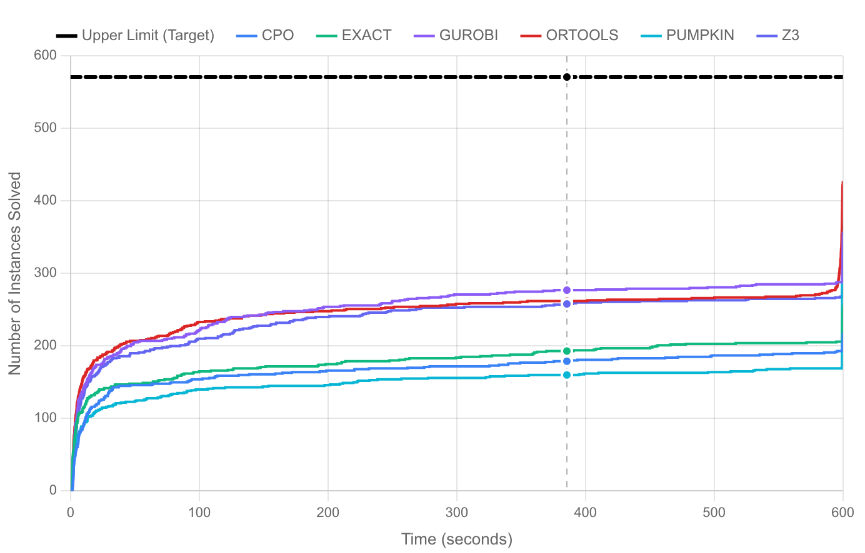
\includegraphics[width=0.3\textwidth]{images/cpmpy_maxsateval2024.png} &
  	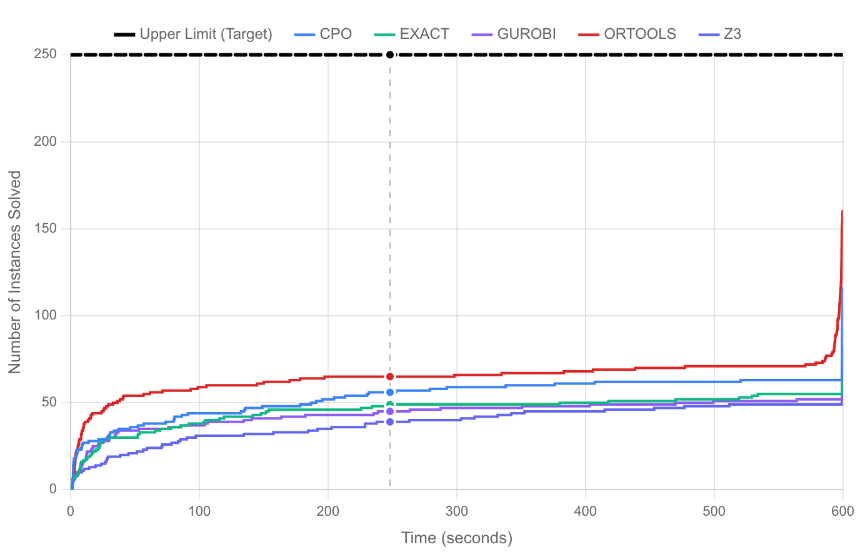
\includegraphics[width=0.3\textwidth]{images/cpmpy_xcsp2024.png} &
  	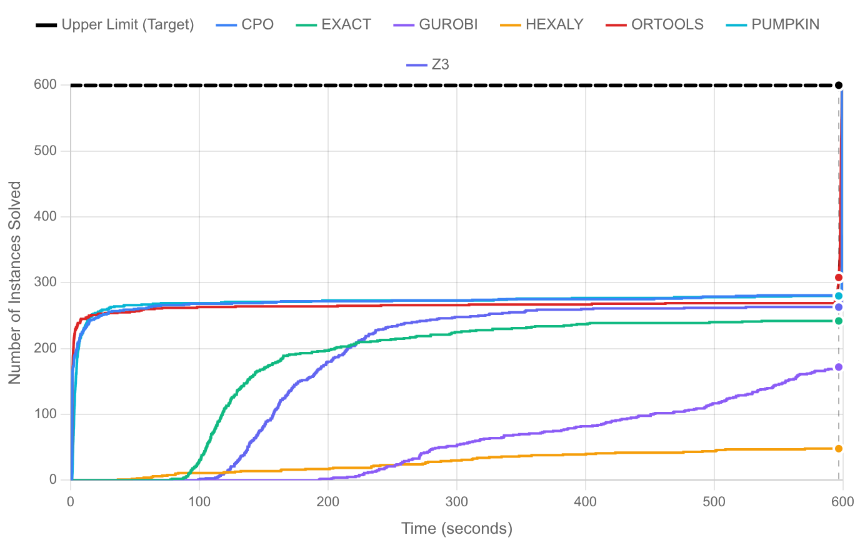
\includegraphics[width=0.3\textwidth]{images/cpmpy_rcspsj120.png} \\
  \end{tabular}
  \pause

  To get more insight, you need to understand
  \begin{itemize}
  	\item What constraints are in your model?
  	\item How close are these constraints to the primitive constraints of the solver \\
  	(= how much \textit{encoding} is needed)
  	\item How well can the solver handle the resulting primitive constraints \\
  	(= how strong do we expect the \textit{inference} to be?)
  \end{itemize}
\end{frame}

\iffalse
% bit too much? rather primitive...
\begin{frame}{How to model in a specific solvers' input language?}
  Every solver has their own input language.
  \vfill

  Different communities have different 'standard' input languages.
  \begin{itemize}
    \item SAT: DIMACS format
    \item Pseudo-Boolean: OPB format
    \item ILP/MIP: MPS format
    \item SMT: SMT-LIB format
  \end{itemize}
  \vspace{1em}

  The CP community does not really have a standard input language (due to the large variety of global constraints possible), BUT it has: \\
  \textbf{solver-independent modelling languages}
  \vfill

  How to go from a high-level modelling language to a specific solver input? Through transformations...
\end{frame}
\fi

\begin{frame}{From Model to Model to Solver: transformations}
\begin{tikzpicture}[scale=0.8, every node/.style={transform shape}, node distance=0.5cm]

\waterfall
\end{tikzpicture}
\end{frame}


\begin{frame}{Goal of the lecture}
	\textbf{Part 1} of solving technologies and encodings: SMT, decomposing global constraints, and CP solving (search + propagation).
	\vfill

	Different solvers will behave differently for different problems...
	\vfill
	
	Typical CP problems are NP-hard, and we can not expect to solve all problems efficiently (unless P=NP).
	\vfill
	
	But many problems of practical interest:
	\begin{itemize}
		\item Can be practically solved
		\item Can be solved even faster with the right solving technology
	\end{itemize}
	\vfill
	\pause
	
	An overview of some solving technologies: \vfill
	\begin{itemize}
	\item to understand their advantages and limitations
	\item to help you choose a technology for a particular model
	\item to help you encode and adapt a model to a particular technology.
	\end{itemize}
	\vfill
	{\small Next lecture (Part 2): flatten nested expressions; ILP, PB, and SAT encodings.}
\end{frame}

\section*{Solvers}

\subsection*{SAT Modulo Theories (SMT)}


% OVERVIEW: SMT solver highlight
\begin{frame}{Overview}
\begin{tikzpicture}[scale=0.7, every node/.style={transform shape}, node distance=0.5cm]

\waterfall[smt2]
\end{tikzpicture}
\end{frame}

\begin{frame}{SMT: SAT Modulo Theories}
	Generalizes SAT solving beyond Boolean variables:	
	\[
	\text{SMT solver} = \text{SAT solver} + \text{Theory solver}
	\]
	\vfill
	
	Used for many \structured{verification} problems (prove a set of statements is True/False):
	
	\begin{itemize}
		\item Verification of hardware designs: Theory of Bit-Vectors
		\item Verification of computer programs: Theory of Arrays
		\item Verification of neural networks: Theory of Real Arithmetic
		\item Security analysis and input validation: Theory of Strings
		\item Transition systems, symbolic executing, planning: Theory of Integer Arithmetic
	\end{itemize}
	\vfill
	
	Many solvers support \textit{theory combination} to combine multiple theories.
	%\vfill
	
	%Can be extended to optimisation, named Optimisation Modulo Theories (OMT)
\end{frame}

\begin{frame}{SMT theories}
	
	\begin{definition}
		A \defined{theory}
		\begin{itemize}
			\item defines theory-specific variables (called a \textit{sort}) and valid \textcolor{blue}{constraint predicates} over those;
			\item is associated with a theory-solver for any conjunction of its
			\textcolor{blue}{predicates}.
		\end{itemize}
	\end{definition}
	\pause
	
	Example formula for the theory of Linear Integer Arithmetic (LIA):
	{\small
	\begin{align*}
		& ((\textcolor{blue}{x < 3}) \lor a) \\
		& (\neg(\textcolor{blue}{x \le 4}) \lor a \lor b) \\
		& (\textcolor{blue}{x \geq 0})\\
		& (\textcolor{blue}{x = y + 1}) \lor (\textcolor{blue}{x \leq 2 \cdot y})
	\end{align*}
	}

	\begin{itemize}
		\item \textbf{Sort:} integers (can be unbounded! unlike in CP) \textit{(here: \textcolor{blue}{$x$} and \textcolor{blue}{$y$})}
		\item \textbf{Constraint predicates:} \textcolor{blue}{linear equalities and inequalities}
		\item \textbf{Theory-solver:} integer linear reasoning
	\end{itemize}
\end{frame}

\begin{frame}{Satisfiability Modulo Theories (SMT)}
	
	There is a standardized language for many different theories, that SMT solvers accept: the SMT-LIB language.
	\vfill
	
	SMT determines the satisfiability of a logical formula over (one or more) background theories.
	\vfill
	
    If SAT: return SAT + a solution to the \emph{theory} problem\\
    If UNSAT: return UNSAT.
    \vfill
    
\end{frame}


\begin{frame}{\textit{Lazy} SMT Solving Architecture\footnote{From: \url{https://users.aalto.fi/\~tjunttil/2020-DP-AUT/notes-smt/lazy.html}}}
	
	\centering
	\scalebox{0.85}{
	\begin{tikzpicture}[
		node distance=0.5cm,
		font=\small,
		every node/.style={align=center},
		box/.style={draw, rounded corners, thick, fill=blue!10, inner sep=4pt},
		satbox/.style={draw, rounded corners, thick, fill=green!15, inner sep=4pt},
		module/.style={draw, rounded corners, thick, fill=green!10, inner sep=4pt},
		arrow/.style={->, thick}
		]
		
		% SMT formula
		\node[box] (smt) {%
			\textbf{SMT formula $\phi$} \\
			{\scriptsize
			$((\textcolor{blue}{x < 3}) \lor a) \land (\neg(\textcolor{blue}{x \le 4}) \lor a \lor b) \land \dots$
			}
		};
		
		% SMT solver box
		\uncover<2->{
			\node[module, below=of smt, text width=15cm, minimum height=5cm] (dpll) {};
			
			\node[anchor=north west, font=\bfseries] at (dpll.north west) {SMT solver};
						
			\node[box, text width=7cm, anchor=north] (propabs) at (dpll.north) {%
				\textbf{Boolean abstraction} \\
				{\scriptsize
					$(\beta_{x<3} \lor a) \land (\neg \beta_{x\le4} \lor a \lor b) \land \dots$
				}
			};
			\draw[arrow] (smt) -- (propabs);
		}
		
		\uncover<3->{
			% SAT solver box
			\node[satbox, below left=0.6cm and 2cm of propabs.south, text width=4.7cm, align=left] (sat) {%
				\textbf{SAT solver} \\[3pt]
				(partial) Boolean assignment \\
				$\neg a, \neg b, \beta_{x<3}, \neg \beta_{x\le4}, \dots$ \\[10pt]
				\only<3-4>{$ $\\$ $} % spacing hack, uncover here gives error
				\only<5->{Conflict clause, forbidding \\the conflict to happen again \\
				$(\neg \beta_{x<3} \lor \beta_{x\le4})$}
			};
			\draw[arrow] (propabs) -- (sat);
		}
	
		\uncover<4->{
			% Theory solver box
			\node[satbox, right=4.1cm of sat.east, text width=4.4cm, align=left] (theory) {%
				\textbf{Theory solver}
				\vspace{2cm}
			};
			
			% SAT-Theory interaction
			\node[above right=1pt and 0pt of sat.east, align=left] (tlits) {\footnotesize Conj. of $T$-literals \\ $(\textcolor{blue}{x < 3}) \land \neg(\textcolor{blue}{x \le 4}) \land \dots$};
			\draw[arrow] ($(sat.east) + (0,5pt)$) -- ($(theory.west) + (0,5pt)$);
		}
			
		\uncover<5->{
			\node[below left=0pt and 0pt of theory.west, align=right] (tconflict) {\footnotesize $T$-\textbf{conflict} \\ $(\textcolor{blue}{x < 3}) \land \neg(\textcolor{blue}{x \le 4})$};
			\draw[arrow] ($(theory.west) + (0,-25pt)$) -- ($(sat.east) + (0,-25pt)$);
		}
		
		\uncover<6->{
			% Loop
			\draw[->, dashed] 
			($(sat.east)+(-2mm,-1mm)$) arc (45:-405:3mm);
		}
		
		\uncover<7->{
			% Solution
			\node[box, below=0.4cm of dpll] (sol) {%
				\textbf{UNSAT or solution}
			};
			\draw[arrow] (dpll) -- (sol);
		}
		
	\end{tikzpicture}
	} % scalebox
\end{frame}

\begin{frame}{\textit{Lazy} SMT Solving Architecture}
	\textbf{Key idea:} combine Boolean level reasoning with theory-specific algorithms.
	\vfill
	
	\structured{Boolean abstraction:}
	\begin{itemize}
		\item Separates the theory constraints from the logic: each theory constraint is represented by a T-literal\footnote{if '$a$' is a Boolean decision variable, then both '$a$' and '$\neg a$' are literals} in the SAT solver.
		\item The result is a pure logic formula over literals (the Boolean abstraction)
	\end{itemize}
	
	\structured{SAT solver:}
	\begin{itemize}
		\item Handles the logic part, including disjunctions of theory constraints
		\item Sends valid (partial) assignments of T-literals to the theory solver for checking
	\end{itemize}
	\pause
	
	\structured{Theory solver:}
	\begin{itemize}
		\item Receives \textit{conjuctions} of T-literals/theory constraints, and checks their validity
		\item If they are theory-satisfiable, can return a solution to the theory variables
		\item If not satisfiable, will return a T-conflict: a subset of T-literals that can not be satisfied together
	\end{itemize}
\end{frame}


\begin{frame}{\textit{Lazy} SMT Solving Architecture, efficiently}
	Additional techniques to make it more efficient:
	\begin{itemize}
		\item The SAT solver will pass T-literals to the theory solver one by one, as soon as it derives them (e.g. through propagation or branching)
		\item The theory solver is \textbf{incremental}: it can incrementally check only the relevant parts of the theory when a T-literal is set
		%\item The theory solver is stateful: it keeps its own \textit{trail} of assigned T-literals, and the SAT solver will inform it when it should backtrack
		\pause
		\item The theory solver tries to return as small a conflict as efficiently possible (helps the SAT solver)
		\pause
		\item The theory solver can be asked for theory-implied literals; for which it can return a clausal explanations (helps the SAT solver)\\
		\textit{(e.g. $\beta_{y > 2}: ~\beta_{x > 2} \land \beta_{y > x} \rightarrow \beta_{y > 2}$, equivalently $\neg\beta_{x > 2} \lor \neg\beta_{y > x} \lor \beta_{y > 2}$ )}
	\end{itemize}	
\end{frame}


\begin{frame}{SMT/OMT for combinatorial problems}
  Theory: QF\_LIA = "Quantifier Free, Linear Integer Arithmetic"
  (and QF\_NIA in case of non-linearities; theory combination comes at a small cost)
  \vfill

  Supports Bool and Int, as well as logical and arithmetic operators; including nested expressions thereof.
  \vfill
  
  No global constraints / global functions in QF\_LIA:
  \begin{itemize}
  	\item requires to \defined{decompose} global constraints
  \end{itemize}
  \vfill
  \pause
  
   OMT (Optimisation Modulo Theories) is an extension for optimisation supported by some SMT solvers
   \vfill
   \pause
   
   Unlike finite-domain CP solvers, SMT solvers are not restricted to finite-domain problems (but this unused generality can have some efficiency cost).
\end{frame}


\subsection*{Transformation: decompose}
\begin{frame}{Overview}
\begin{tikzpicture}[scale=0.7, every node/.style={transform shape}, node distance=0.5cm]

\waterfall[decompose]
\end{tikzpicture}
\end{frame}

\begin{frame}{Decomposition of unsupported globals}

	For \textbf{global constraints}: replace it by its decomposition.\\
	Example: $\cons{AllDifferent}{u,v,w} \Longrightarrow u \neq v \land u \neq w \land v \neq w$
	\vfill
	
	For \textbf{global functions}, used in a numeric expression:
	\pause
	\begin{itemize} 	
		\item<2> The classic view is that you can replace the global function by a fresh auxiliary variable, and add the functional global constraint, or rather its decomposition, over the auxiliary as a new constraint.
		\vfill
		
		\item<3> We can alternatively separate a global function decomposition into a '\textcolor{blue}{value}' expression and a set of '\textcolor{purple}{defining}' constraints. We then replace the global function by the '\textcolor{blue}{value}' expression, and add the '\textcolor{purple}{defining}' constraints as new constraints.
	\end{itemize}
	\only<2>{
		Example: $\cons{Count}{X, 0} \geq 2$ \\
		$\quad \quad \quad ~\equiv~ a \geq 2 ~\land~ \cons{CountEq}{X, 0, a}$ \\
		$\quad \quad \quad ~\equiv~ a \geq 2 ~\land~ a = \sum_{i} \Iverson{X_i = 0}$
	}
	\only<3>{
		Example 1: $\cons{Count}{X, 0} \geq 2 ~\equiv~ \textcolor{blue}{\sum_{i} \Iverson{X_i = 0}} \geq 2$ (no defining constraints) \\
		Example 2: $\cons{Nvalue}{X} \geq 2 ~\equiv~ \textcolor{blue}{\sum_{v} B_v} \geq 2 ~\land~ \textcolor{purple}{\forall v \in V: B_v = \bigvee_{i} ( X_i = v )} $
	}
\end{frame}



\begin{frame}{Decomposition and negation}
	If we also want to support \textbf{negating global constraints}, then we have to be more careful!
	\vfill
	
	If a \textbf{global constraint} decomposition introduces new auxiliary variables, we can not simply negate the decomposition.
	\vfill
	
	\only<1>{
	\begin{example}
		Imagine a global constraint \cons{Equals2}{x} with decomposition $x = a \land a = 2$, e.g. it uses an auxiliary variable to ensure $x$ equals 2.
		
		If we have constraint $\neg \cons{Equals2}{x}$ we can not simply replace the subexpression by its decomposition.\\
		If we would, we would get $\neg (x = a \land a = 2)$ which equals $(x \neq a) \lor (a \neq 2)$ hence $x=2$ would be a valid solution as $a$ can just take any value other than 2.
	\end{example}
	}
	
	\only<2>{
	A \underline{solution} is also for global constraints to separate its decomposition into a (Boolean) '\textcolor{blue}{value}' expression and a set of '\textcolor{purple}{defining}' constraints.
	\vfill
	Then we must do the following:
	\begin{enumerate}
		\item we replace the global constraint by the \textcolor{blue}{value expression}
		\item we add the \textcolor{purple}{defining constraints} directly to the solver (always enforced)
	\end{enumerate}
	\vfill
	In our example case $\cons{Equals2}{x} ~\equiv~ \textcolor{blue}{x=a} \land \textcolor{purple}{a=2}$,\\
	So then $\left(y \lor \neg \cons{Equals2}{x}\right)$ \\
	$\quad \quad ~\equiv~ \left(y \lor \neg \textcolor{blue}{(x=a)}\right) \land \textcolor{purple}{a=2}$
	}
\end{frame}

\begin{frame}%{Decomposition and negation}
	
	For \textbf{global functions} we also need to be careful if it is a \textbf{partial function} AND if it is used within a reified expression or negation.
	\vfill
	
	A global function is \defined{partial} if its value is undefined for some assignment to its decision variables.
	
	The following 3 global functions can be partial:
	\begin{itemize}
		\item Integer division $x / y$: undefined when $y=0$
		\item Modulo $x ~\text{mod}~ y$: undefined when $y=0$
		\item Element $Arr[idx]$: undefined when $idx$ is not in the range of $Arr$
	\end{itemize}
	\vfill
	\pause
	
	A \underline{solution} is to transform the reified/negated partial function into a modified reified/negated \textit{safened} total function, following the \textit{relational semantics}.
	\vfill
	
	Fine details: \textit{\footnotesize Alan Frisch and Peter J. Stuckey. "The proper treatment of undefinedness in constraint languages." CP 2009}, \\
	Implementation: {\tiny \url{https://cpmpy.readthedocs.io/en/latest/api/transformations/safening.html}}
\end{frame}

\begin{frame}{Decomposition, example}
	Rewrite global constraints \textit{that the solver does not support}, using (more) primitive constraints. For SMT: all globals.
	\vfill
	
	Example constraint model:
	\begin{align*}
		&\cons{AllDifferent}{x,y,z} \\
		&(x = 3) \rightarrow (y + z <= 3) \\
		&x,y,z \in \{1,2,3\}
	\end{align*}
	\vfill
	
	After transformations:
	\begin{align*}
		&x \neq y \land x \neq z \land y \neq z \\
		&(x = 3) \rightarrow (y + z <= 3) \\
		&x,y,z \in \{1,2,3\}
	\end{align*}
\end{frame}


\subsection*{Constraint Programming (CP)}


% OVERVIEW: CP solver highlight
\begin{frame}{Overview}
\begin{tikzpicture}[scale=0.7, every node/.style={transform shape}, node distance=0.5cm]

\waterfall[cp2]
\end{tikzpicture}
\end{frame}


\begin{frame}{CP: Constraint Programming}
	For \textit{finite-domain} combinatorial search problems:	
	\[
	\text{CP} = \text{\inference{propagation}} + \text{\search{search}}
	\]
	\vfill
	
	Includes logical, arithmetic and specialised \textit{global constraints}. Solves both satisfaction and optimisation problems.
	\vfill
	
  \textbf{Typical Applications}
  \begin{itemize}
    \item Scheduling, Timetabling, Assignment problems
    \item Routing Problems, Packing problems, esp. with side-constraints
    \item Puzzles and Games, Configuration Problems
  \end{itemize}
\end{frame}

\begin{frame}{Domains}
  Central concept: the \textbf{domain store}
  
  \begin{definition}
    The \defined{domain} of a decision variable $v$, denoted by
    $\Domain{v}$, is the set of values that $v$ can still take during
    \search{search}:
    \begin{itemize}
    	\item A domain can only be \textbf{reduced}, by \search{search} and \inference{propagation}
    	\item A decision variable is said to be \defined{fixed} if its
    	domain is a singleton.
    	\item \defined{Unsatisfiability} occurs if the domain of a
    	decision variable becomes empty,\\
    	search then backtracks (and restores the domains)
    \end{itemize}
  \end{definition}
  \vfill
  \pause

  Each individual constraint will \inference{propagate} independently: it can read from the domain store, and reduce domains in the domain store.
  \vfill
  
  Recap example: $x + 2 \cdot y \geq 3, \quad D(x) = \{0,1,2\}, D(y) = \{0,1,2\}$ \\
  $\qquad \qquad \qquad \implies D(y) = \{\cancel{\red{0}},1,2\}$
\end{frame}


\begin{frame}{CP solver architecture, propagator view}
  \centering
  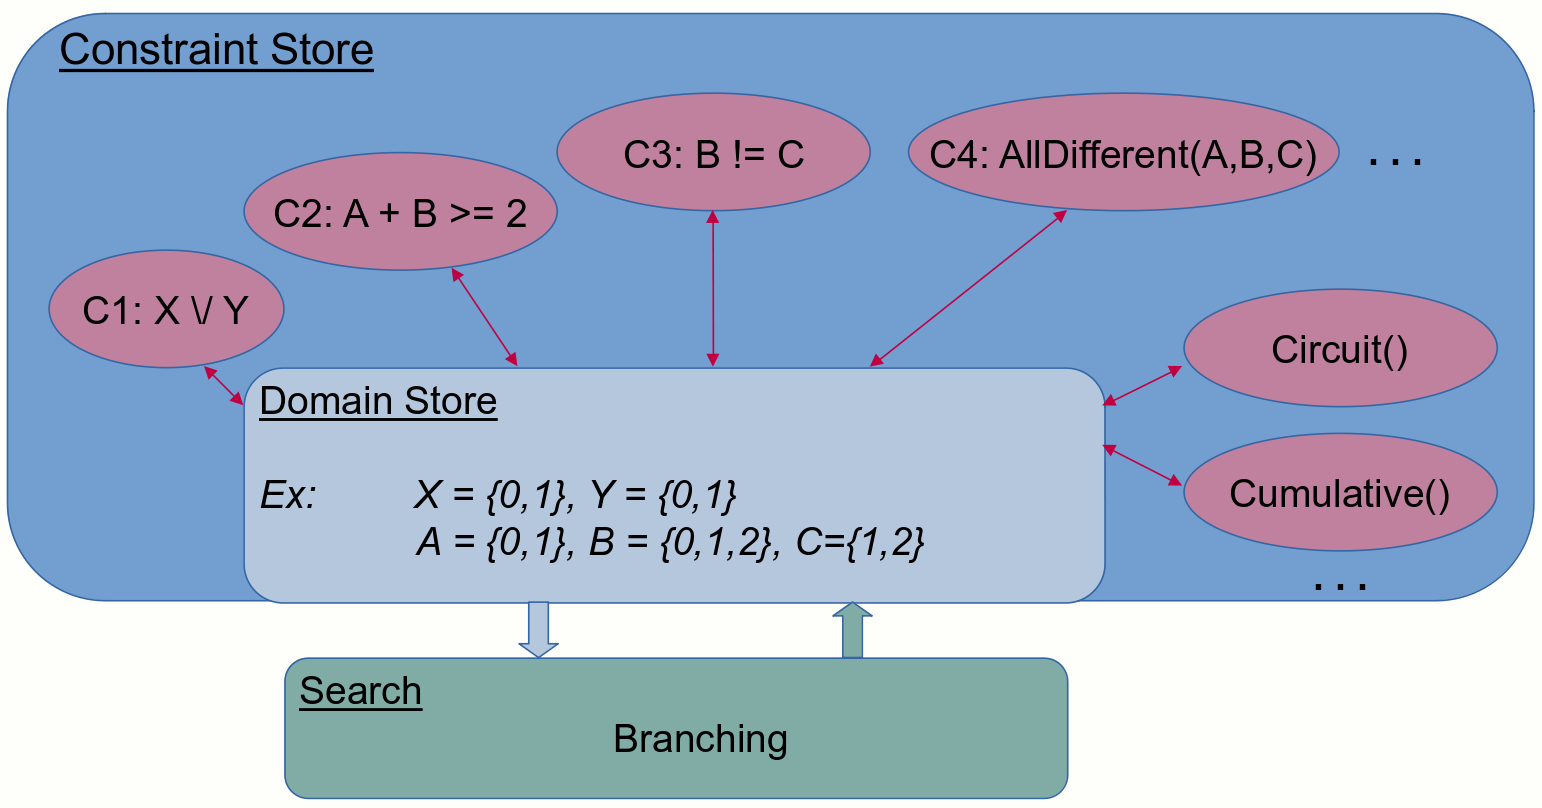
\includegraphics[height=70mm]{images/cp_domain_store.png}
\end{frame}

\begin{frame}{CP solver architecture, search tree view}
	\begin{itemize}
		\item Initialize the domain store with the initial domain
		\item<2-> Each constraint \textbf{propagator} gets the current domain as input, and outputs the same or a \textit{reduced} domain
		\item<3-> If all propagators are at \textbf{fixpoint} (their output=their input): create a \search{\textbf{branch}} in the search tree by choosing a non-fixed variable $V$ and choosing a value $v \in D(V)$, and fixing the variable to this value: $D(V) = v$. \\
		\item<4-> On \textbf{backtracking} over this choice, restore to the previous $D(V)$ and enforce $V \neq v$ to explore the other branch\footnote{This creates a binary search tree, one can also branch over each value in $D(V)$ in turn}.
		\item<5-> If a propagator returns an empty domain for a decision variable: \textbf{fail and backtrack}
		\item<6-> If all variables are \textit{fixed} (have a singleton value): \textbf{return} the found solution.
	\end{itemize}
	
	% --- Place the small search tree in the top-right corner ---
	\begin{tikzpicture}[remember picture, overlay, scale=0.7, every node/.style={transform shape}]
		\node[anchor=north east] at ([xshift=-0.5cm,yshift=-0.3cm]current page.north east) {
			\begin{tikzpicture}[
				xnode/.style={draw, circle, minimum size=4mm, inner sep=1pt},
				xlabel/.style={font=\scriptsize},
				level distance=10mm,
				sibling distance=12mm
				]
				\node[xnode] (root) {}
				child[visible on=<3->] { node[xnode, alt=<3>{solid}{dashed}] (L) {}
					edge from parent[alt=<3>{draw}{draw,dashed}] node[xlabel, left, midway] {$V=v$}
				}
				child[visible on=<4->] { node[xnode] (R) {}
					child[visible on=<5->] { node[xnode, alt=<5>{solid}{dashed}] (RL) {}
						edge from parent[alt=<5>{draw}{draw,dashed}] node[xlabel, left, midway] {$W = w$} }
					child[visible on=<6->] { node[xnode] (RR) {}
						edge from parent node[xlabel, right, midway] {$W \neq w$} }
					edge from parent node[xlabel, right, midway] {$V\neq v$}
				};
				% --- Dashed self-loops placed slightly to the left of each node ---
				\path (root.west); % get coordinate
				% draw a small loop offset to the left
				\draw[dotted,->,visible on=<2->] ([xshift=-2pt,yshift=2pt]root.west)
				arc[start angle=60, end angle=320, radius=3pt];
				\draw[dotted,->,visible on=<3->] ([xshift=-2pt,yshift=2pt]L.west)
				arc[start angle=60, end angle=320, radius=3pt];
				\draw[dotted,->,visible on=<4->] ([xshift=-2pt,yshift=2pt]R.west)
				arc[start angle=60, end angle=320, radius=3pt];
				\draw[dotted,->,visible on=<5->] ([xshift=-2pt,yshift=2pt]RL.west)
				arc[start angle=60, end angle=320, radius=3pt];
				\draw[dotted,->,visible on=<6->] ([xshift=-2pt,yshift=2pt]RR.west)
				arc[start angle=60, end angle=320, radius=3pt];
				%\foreach \n in {root,L,R,RL,RR} {
				%	\path (\n.west); % get coordinate
				%	% draw a small loop offset to the left
				%	\draw[dashed,->] ([xshift=-2pt,yshift=2pt]\n.west)
				%	arc[start angle=60, end angle=320, radius=3pt];
				%}
			\end{tikzpicture}
		};
	\end{tikzpicture}
\end{frame}

\begin{frame}{Propagation of constraints, more formally}
  \begin{definition}
    A \inference{propagator} for a constraint $\gamma$ deletes from the
    domains of the decision
    variables of a~$\gamma$-constraint,
    the values that cannot
    be in a solution to that constraint. \\
  \end{definition}
  \begin{examples}
    \begin{itemize}
      \item For $x < y$: when $\Domain{x} = \{1..4\}$ and $\Domain{y} = \{-1..3\}$,
        delete $\{3, 4\}$ from $\Domain{x}$ and
        $\{-1..1\}$ from $\Domain{y}$.
      \item For $\cons{AllDifferent}{x,y,z}$: when
        $\Domain{x} = \{1,3\}$ =
        $\Domain{y}$ and $\Domain{z} = \{1..4\}$, delete $1$ and $3$ from
        $\Domain{z}$ so that it becomes the non-range
        $\{2,4\}$.
    \end{itemize}
  \end{examples}
\end{frame}


\begin{frame}{Propagation strength}\label{propagator}
	The more values a propagator can remove, the fewer search we have to do, \\
	but propagation also takes computation time!
	\vfill
	\pause
	
	The propagation strength of a propagator can be expressed in terms of the \defined{consistency} that it achieves:
	\begin{definition}
		\begin{itemize}
			\item \underline{Arc consistency}, for constraints between two variables A and B:\\
			For each value v in A, there is a value w in B such that the constraint is satisfied, and vice-versa.
			
			\item \underline{Generalised arc consistency} (GAC), or domain consistency: \\
			every value in every variable exists in at least one solution to the
			constraint.
			
			\item \underline{Bounds consistency}: the upper and lower bounds of every
			variable exist in at least one solution to the constraint.
		\end{itemize}
	\end{definition}
	\vfill
	\pause
	
	(there exist more forms of consistency, but GAC/Bounds are the most important)
\end{frame}

\begin{frame}{Propagation strength}
	\begin{example}[Linear equality constraints]
		Consider the linear constraint $3 \cdot x + 4 \cdot y = z$ \\
		with $\Domain{x} = \Set{0,1} =
		\Domain{y}$ and $\Domain{z} =
		\Set{0,\dots,10}$:
		\begin{itemize}
			\item A bounds consistent propagator reduces
			$\Domain{z}$ to $\Set{0,\dots,7}$.
			\item A GAC propagator reduces
			$\Domain{z}$ to $\Set{0,3,4,7}$.
		\end{itemize}
		\vfill
		
		\textbf{Time complexity:}
		\begin{itemize}
			\item A bounds consistent propagator for a linear equality
			constraint can be implemented to run in $\Oh{n}$ time, where $n$
			is the number of decision variables in the constraint. 
			\item A GAC propagator for a linear equality
			constraint can be implemented to run in $\Oh{n \cdot d^2}$ time,
			where $n$ is the number of decision variables in the constraint
			and $d$ is the sum of their domain sizes.
			% TODO: I'm not actually sure why nd2?
			%, hence in time pseudo-polynomial = exponential in the input magnitude.
		\end{itemize}
	\end{example}
	
\end{frame}


\begin{frame}{CP solver architecture, efficiency?}
	\centering
	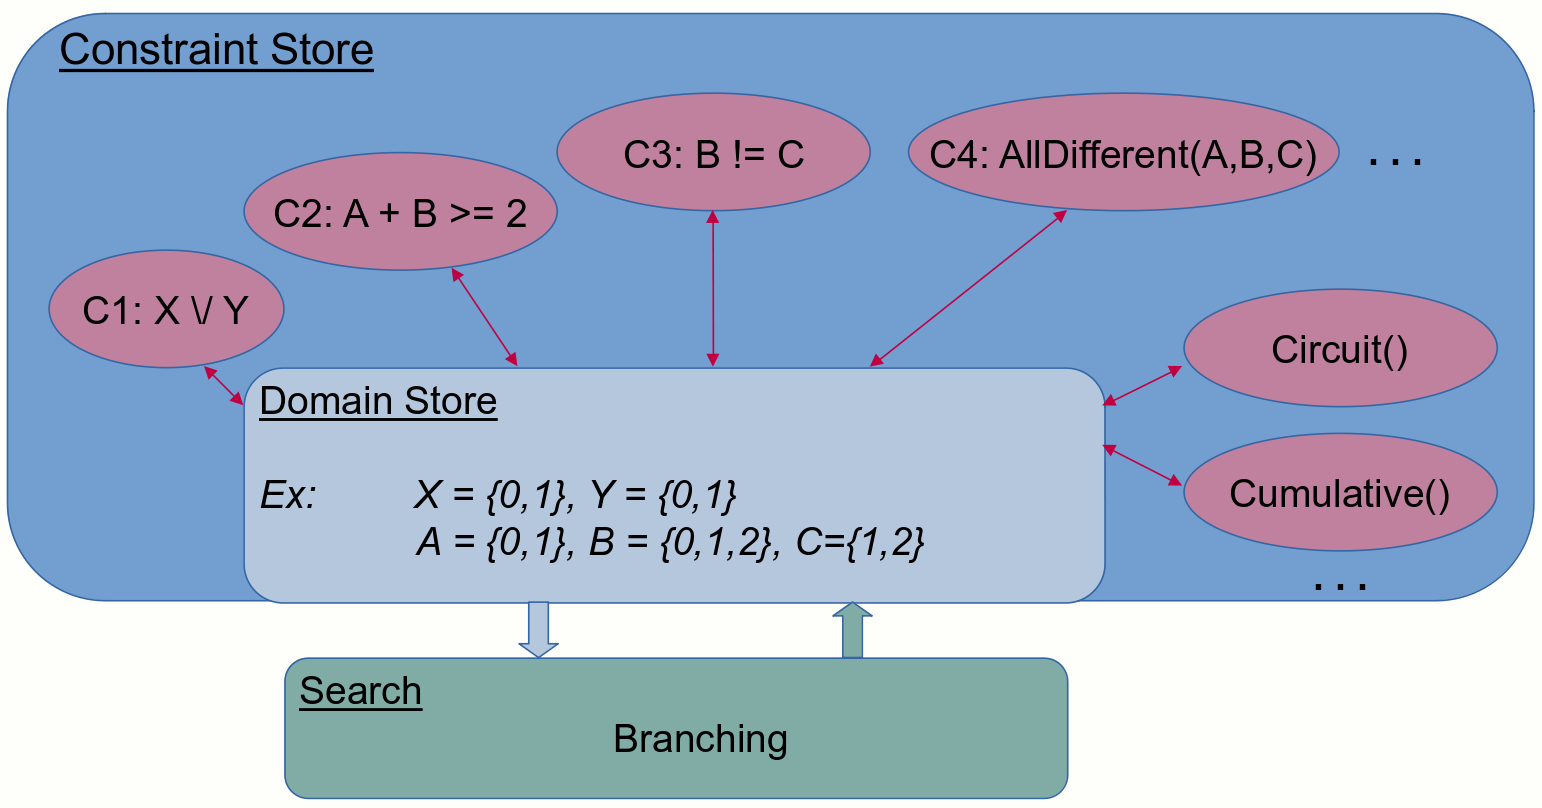
\includegraphics[height=70mm]{images/cp_domain_store.png}
\end{frame}

\begin{frame}{Efficient CP solvers, fixpoint algorithm}
	
	% --- Place the figure in the top-right corner ---
	\begin{tikzpicture}[remember picture, overlay,
		shift={(current page.north east)}, xshift=-1cm, yshift=-1cm, scale=0.7,
		every node/.style={circle, draw, minimum size=8pt, inner sep=0pt}]
		% Left nodes (C)
		\node[draw=none] (Clabel) at (-1,1) {$C$};
		\foreach \i in {1,...,3}
		\node (c\i) at (-1, 0.8-\i*0.8) {};
		% Add vertical dots below c3
		\node[draw=none] at (-0.99, -2.2) {\small $\vdots$};
		
		\only<2->{
		% Right nodes (V)
		\node[draw=none] (Vlabel) at (1,1) {$V$};
		\foreach \i in {1,...,4}
		\node (v\i) at (1, 1.2-\i*0.8) {};
		
		
		% Connections
		\draw (c1) -- (v1);
		\draw (c1) -- (v2);
		\draw (c2) -- (v1);
		\draw (c2) -- (v3);
		\draw (c3) -- (v2);
		\draw (c3) -- (v3);
		\draw (c3) -- (v4);
		}
	\end{tikzpicture}
	
	Avoiding propagator calls in the fixpoint propagation loop.
	\vfill
	\pause
	
	Only wake up when one of your variables changed \only<3->{(meaningfully)}
	\begin{itemize}
		\item Each variable has a \textit{watch-list} of constraints that 'watch' it for domain change,\\
		only those are added to the propagator queue, until the queue is empty
		\vfill
		\pause
		
		\item In many solvers, propagators can register for specific domain events (e.g. only bound(s) or only when a variable is fixed) \\
		\textit{Example: the $X \neq Y$ constraint can only propagate when a variable is fixed.}
		\vfill
		\pause
		
		\item Often the queue has buckets so that 'cheaper to propagate' constraints are checked before more expensive ones\\
		(because the sooner you check it, the higher the chance it is re-added to the queue when one of its variables change)
	\end{itemize}
	
	
\end{frame}

\begin{frame}{Efficient CP solvers, incremental state}
	
	% --- Place the small search tree in the top-right corner ---
	\begin{tikzpicture}[remember picture, overlay, scale=0.7, every node/.style={transform shape}]
		\node[anchor=north east] at ([xshift=-0.5cm,yshift=-0.3cm]current page.north east) {
			\begin{tikzpicture}[
				xnode/.style={draw, circle, minimum size=4mm, inner sep=1pt},
				xlabel/.style={font=\scriptsize},
				level distance=10mm,
				sibling distance=12mm
				]
				\node[xnode] (root) {}
				child { node[xnode] (L) {}
					child { node[xnode] (LL) {}
						edge from parent node[xlabel, left, midway] {$W = w$} }
					child { node[xnode] (LR) {}
						edge from parent node[xlabel, right, midway] {$W \neq w$} }
					edge from parent node[xlabel, left, midway] {$V=v$}
				}
				child { node[xnode] (R) {}
					edge from parent node[xlabel, right, midway] {$V\neq v$} };
				% --- Dashed self-loops placed slightly to the left of each node ---
				\foreach \n in {root,L,R,LL,LR} {
					\path (\n.west); % get coordinate
					% draw a small loop offset to the left
					\draw[dashed,->] ([xshift=-2pt,yshift=2pt]\n.west)
					arc[start angle=60, end angle=320, radius=3pt];
				}
			\end{tikzpicture}
		};
	\end{tikzpicture}
	
	\vfill
	Each propagator is \textbf{incremental}: only checks what has changed, and can keep its own (backtrackable) state.
	\vfill
	\pause
	
	
	Efficient backtracking:\\
	before branching, make a '\textbf{save point}' of the domains and propagator states, and restore to that save point on backtracking.
	\begin{itemize}
		\item<3-> \underline{Copying:} copy the state before making a change, replace the original on backtracking
		\item<4-> \underline{Trailing (most solvers):} keep a list of restoring operations: when making a change, record how to undo the change; on backtracking, undo the changes
	\end{itemize}
	\vfill
	\pause
	
	\only<5->{Lots of research goes into developing highly efficient, incremental propagators for global constraints!}
	
	
\end{frame}

\subsubsection{Search strategies}

\begin{frame}{Search Strategies}\label{searchCP}
	CP Search is almost always \textbf{depth-first search} (with efficient backtracking).
	\vfill
	
	\search{Branching decisions:}
	\begin{itemize}
		\item Which decision variable to branch on?
		\item Which value to branch on first?
	\end{itemize}
	\vfill
	\pause
	
	Goal: explore the search space as efficiently as possible.
	\vfill
	
	Can we \textit{cheaply} estimate the quality of a branching decision? $\rightarrow$ \defined{branching heuristics} 
\end{frame}

\begin{frame}{Variable Selection Heuristics: Min-Dom}
	\begin{example}[Impact of domain size on search tree size]
		Consider $x \in \Set{1,2}$, $y \in \Set{1,2,3,4}$, $z \in \Set{1,\dots,6}$

		\begin{itemize}
			\item If selecting the decision variables in the order
			$x, y, z$, \\
			the search tree has 
			$1 + 2 + 2 \cdot 4 + 2 \cdot 4 \cdot 6 = $ \textbf{59}
			nodes. \\
			\only<1>{
			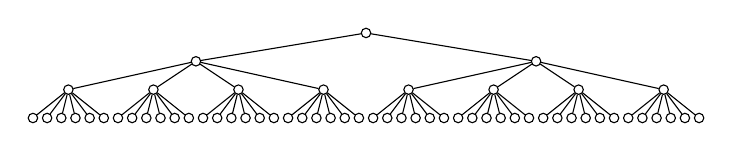
\begin{tikzpicture}[ scale=0.6, transform shape,
				level distance=6mm,
				every node/.style={circle, draw, inner sep=1pt, minimum size=2mm},
				level 1/.style={sibling distance=72mm},
				level 2/.style={sibling distance=18mm},
				level 3/.style={sibling distance=3mm}
				]
				\node {}
				child foreach \a in {1,2} { node {}
					child foreach \b in {1,2,3,4} { node {}
						child foreach \c in {1,2,3,4,5,6} { node {}
						}
					}
				};
			\end{tikzpicture}
			}
			
			\item If selecting the decision variables in the order
			$z, y, x$, \\
			the search tree has
			$1 + 6 + 6 \cdot 4 + 6 \cdot 4 \cdot 2 = $ \textbf{79}
			nodes. \\
			\only<1>{	
			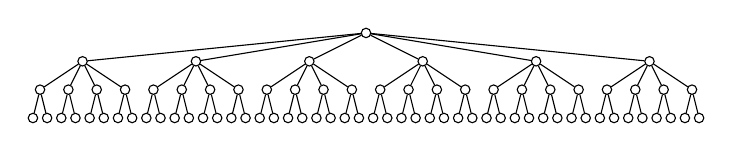
\begin{tikzpicture}[ scale=0.6, transform shape,
				level distance=6mm,
				sibling distance=4mm,
				every node/.style={circle, draw, inner sep=1pt, minimum size=2mm},
				level 1/.style={sibling distance=24mm},
				level 2/.style={sibling distance=6mm},
				level 3/.style={sibling distance=3mm}
				]
				\node {}
				child foreach \a in {1,2,3,4,5,6} { node {}
					child foreach \b in {1,2,3,4} { node {}
						child foreach \c in {1,2} { node {}
						}
					}
				};
			\end{tikzpicture}
			}
		\end{itemize}
	\end{example}
	\vfill
	\pause
	
	Ignoring propagation, multi-way branching over variables with small domains higher in the tree leads to fewer internal search nodes.
	\vfill
		
	Dom heuristic (select smallest): $|D(V)|$ \quad \textit{(cardinality/size of the set $D(V)$)}
\end{frame}

\begin{frame}{Variable Selection Heuristics: Min-Dom/Deg}
	
	\defined{Degree} of a decision variable $V$: the number of constraints that the variable is involved in.
	\vfill
	
	Dom/Deg heuristic (select smallest): $\dfrac{|D(V)|}{Deg(V)}$
	\vfill
	
	Idea: prefer small domains (smaller tree), but also variables that are involved in many constraints (higher chance to fail).
	\vfill
	
	\textbf{First-fail principle:} if a decision leads to a fail, it is better to have it early in the search tree, to allow the pruning of many children nodes \footnote{[Increasing tree search efficiency for CSPs, by R. Haralick and G. Elliott, IJCAI 1979]}
\end{frame}


\begin{frame}{Variable Selection Heuristics: Activity-based search}
	
	Can we capture how actively a decision variable is contributing to search space reductions?
	\vfill
	
	Idea: propagation shrinks domains, hence recent domain changes indicate potentially important variables.
	\vfill
	
	Variable activity with decay:
	\begin{itemize}
		\item Initialize an activity value $A(V)$ for each variable
		\item After propagation reaches fixed-point:
		\begin{itemize}
			\item decay each activity by $\alpha$: $A(X) = \alpha \cdot A(X)$
			\item set $A(V) = A(V)+1$ if $D(V)$ has been modified
		\end{itemize}
	\end{itemize}
	\vfill
	Activity-based search heuristic (select largest): $\dfrac{A(V)}{|D(V)|}$
\end{frame}

\begin{frame}{Variable Selection Heuristics: Conflict ordering search}
	
	Can we directly capture how often a variable is involved in a conflict?
	\vfill
	
	Idea: if a branching decision results in propagation discovering a failure, then \textbf{timestamp} the variable branched on.
	\vfill
	
	Conflict ordering search heuristic (select largest): $\text{timestamp}(V)$
\end{frame}


\begin{frame}{Impact of search heuristics}
	\begin{example}
		Finding the first solution to $250$-queens with CPMpy-Choco
		(CP):
		\begin{center}
			%% on Tias' intel laptop, Nov 2024
			\begin{tabular}{lrr}
				search & seconds \\
				\midrule
				default & 0.17 \\
				min-dom, lb value & 0.19 \\
				conflict-ordering search & 0.22 \\
				activity-based search & 0.23 \\
				dom over (weighted)degree & $>30$ \\
				input order, lb value & $>30$ \\
				%failure rate-based search & >30
			\end{tabular}
		\end{center}
	\end{example}
	
	Note: value ordering heuristics also exist (e.g. lowerbound, upperbound, mid...)
\end{frame}

\iffalse
\begin{frame}{Value ordering heuristics}
	\begin{definition}[Best-First Principle]
		First try a domain part that is most likely, if not guaranteed, to
		have values that lead to solutions.
	\end{definition} \vfill%
	
	This may be like how one would make the greedy choice in a greedy
	algorithm for the problem at hand, considering its objective
	function.
	
	\begin{example}[Impact of the domain partitioning strategy]
		%(Continued from slide~\ref{var}) \\ 
		Finding the first solution to $750$-queens with CPMpy-Choco
		\begin{center}
			%% on Tias' intel laptop, Nov 2024
			\begin{tabular}{lrr}
				search & seconds \\
				\midrule
				smallest-domain, lb value & 3.35 \\
				smallest-domain, ub value & 2.88 \\
			\end{tabular}
		\end{center}
	\end{example}
\end{frame}
\fi

\begin{frame}{Search heuristics in CP: historic perspective}
	
	Historically, constraint programming solvers allow programming your own constraints as well as \defined{programmable search}:
	\vfill
	
	Using your domain knowledge to determine variable/value ordering and choices, e.g. which variables, what branching decision are created... also full access to the constraint, domain store and solver statistics.
	
	\textbf{$\rightarrow$ CP as a generic depth-first search \textit{framework}}
	\vfill
	
	Since a number of years, the CP community has been advancing on \textbf{black box} search strategies that work well in general (e.g. activity \& conflict based search). %, so users can especially focus on the modeling part.
	\pause
	
	\textbf{$\rightarrow$ CP as generic satisfaction/optimisation \textit{solver}}
	\vfill
	
	%Solver-indendent modeling languages have taken one step further away from programmable search, allowing setting at most a variable/value ordering as a solver parameter.
\end{frame}

\begin{frame}{CP Solving, optimisation}
	CP is used for both satisfaction and optimisation problems.
	\vfill
	
	In case of \textit{optimisation problems} we assume the presence of an objective function $O(V)$ over a (subset of) the decision variables.
	\vfill
	\pause
	
	Most common technique: \textbf{solution-improving search}:
	\begin{enumerate}
		\item Find any satisfying solution
		\item Compute the objective value $o$ and add the solution-improving constraint $O(V) < o$ (in case of a minimisation problem)
		\item Continue searching, repeat
	\end{enumerate}
	\vfill
	\pause
	
	This will find a sequence of satisfying solutions and finally return UNSAT. The last solution found before that is an optimal solution.\\
	(the solver proved no better solution exists)
\end{frame}

\iffalse
% What actually are 'common' preprocessing steps for CP?
\begin{frame}{Efficient CP solvers, preprocessing}
	Additional techniques to make it more efficient:
	\vfill
	
	\begin{description}
		\item[local search] to quickly find a feasible solution.\\
		Provides an upper bound (for minimisation problems), good user experience
		\vfill
		
		\item[probing\hfill] try assigning a Boolean variable to a value and propagate it (no search), derives failing values and hidden implications
		\vfill
		
		\item[solution hints] if possible, the user can indicate what value to try first for specific variables (useful in repeated solving, e.g. a previous assignment)
		
		% NOT EXPLAINED clause learning solver yet
		%\item[restarts during search] for clause learning solvers, backjump to the root node.\\
		%Can be very effective (because variable activity was updated during previous search, so most active variables are now at 'top' of the tree)
	\end{description}
\end{frame}
\fi

\begin{frame}{Next lecture}
	How to flatten nested expressions to primitive CP constraints.
	\vfill
	
	Lower-level, but highly optimized solver techniques:
	\begin{itemize}
		\item Integer Linear Programming
		\item Pseudo-Boolean solving
		\item Boolean Satisfiability (CDCL)
	\end{itemize}
	
	%After that: portfolio solvers and algorithm configuration.
\end{frame}
\end{document}
